\documentclass[border=12pt]{standalone}
\usepackage[T1]{fontenc}\usepackage[utf8]{inputenc}
\usepackage{helvet}\renewcommand{\familydefault}{\sfdefault}
\usepackage{tikz}\usetikzlibrary{positioning,arrows.meta,shapes.geometric,shapes.symbols,backgrounds,fit,calc}
\definecolor{ing}{HTML}{EA580C}\definecolor{ingbg}{HTML}{FFF7ED}
\definecolor{spk}{HTML}{4F46E5}\definecolor{spkbg}{HTML}{EEF2FF}
\definecolor{hdf}{HTML}{059669}\definecolor{hdfbg}{HTML}{ECFDF5}
\definecolor{rst}{HTML}{DB2777}\definecolor{rstbg}{HTML}{FDF2F8}
\definecolor{ink}{HTML}{1F2937}\definecolor{mut}{HTML}{6B7280}\definecolor{hot}{HTML}{DC2626}
\begin{document}
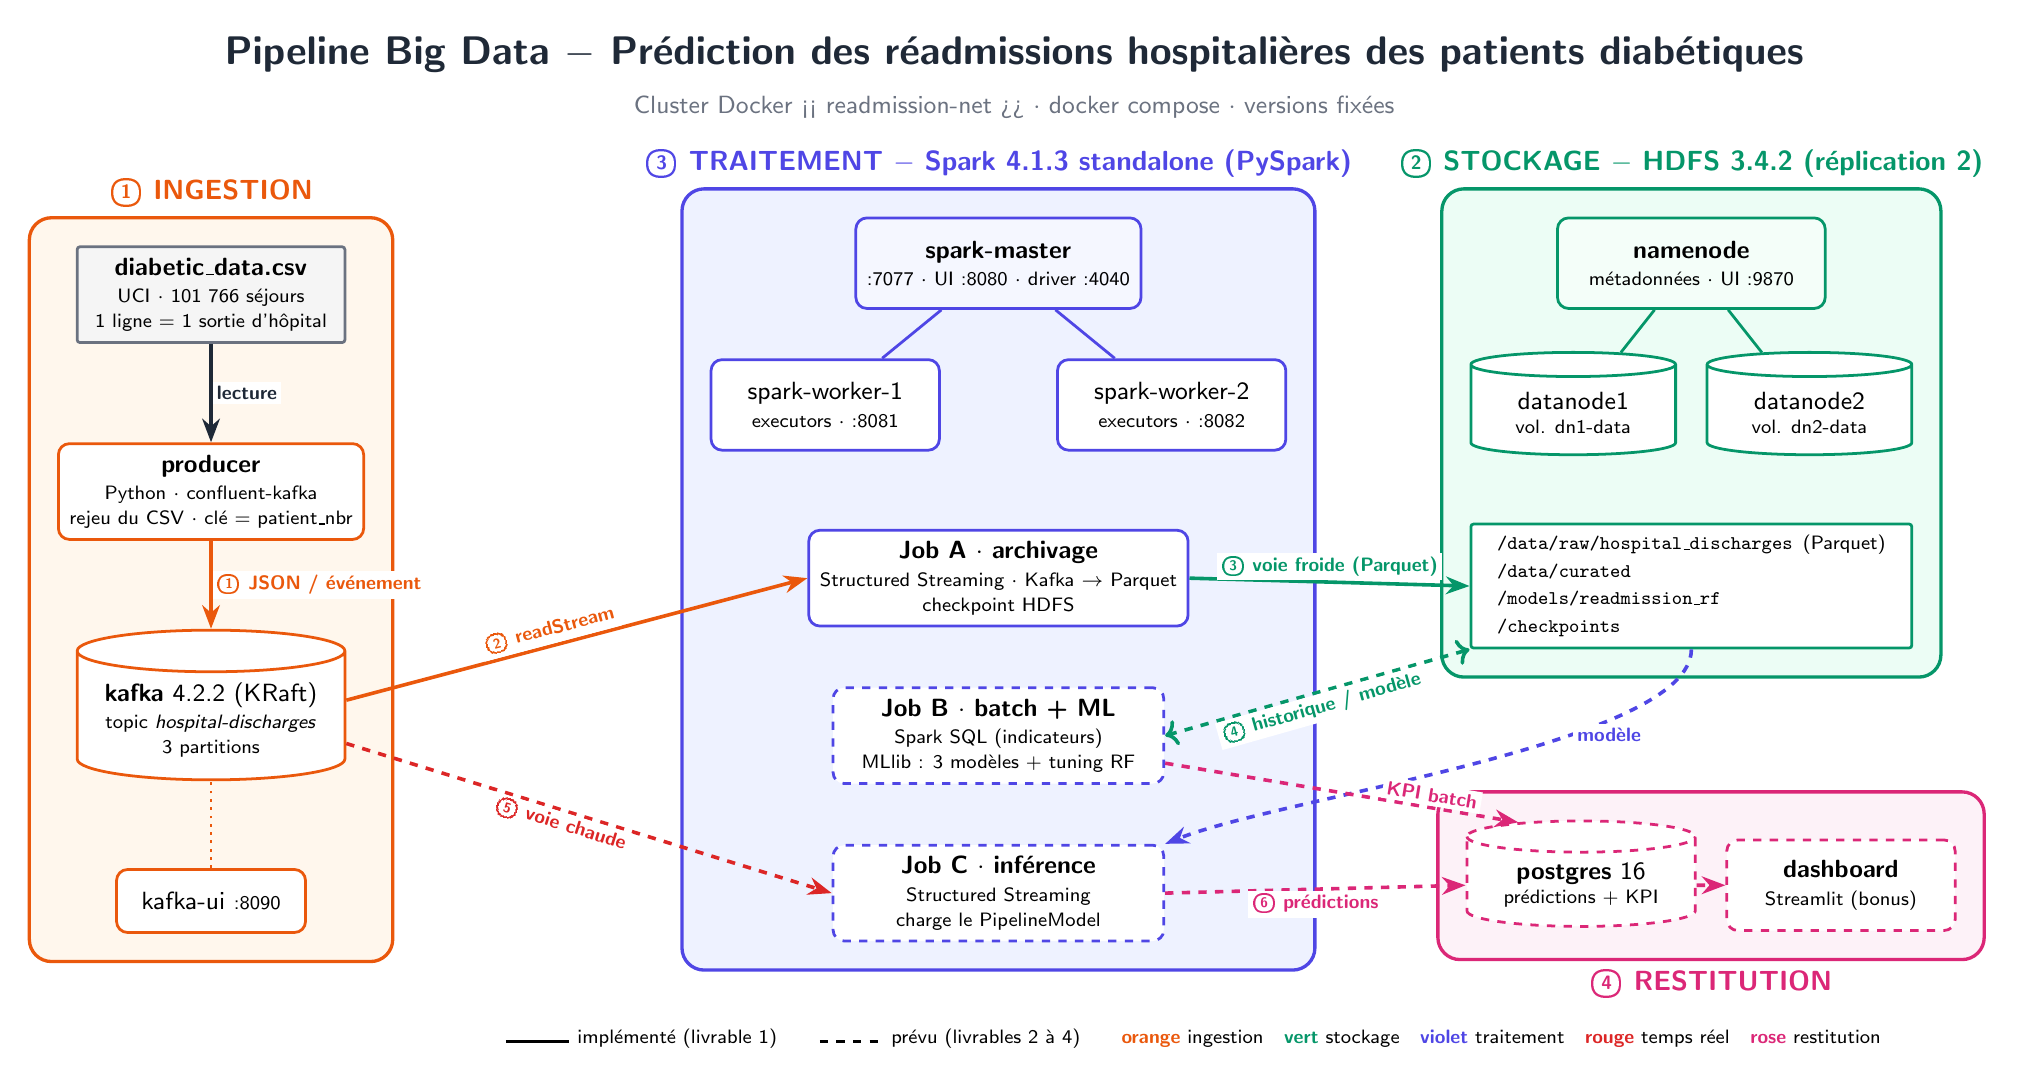
\begin{tikzpicture}[font=\small,
  n/.style={draw=#1,fill=white,rounded corners=4pt,line width=1pt,align=center,minimum width=3.4cm,minimum height=1.15cm,inner sep=4pt},
  p/.style={n=#1,dashed},
  cyl/.style={cylinder,shape border rotate=90,aspect=0.18,draw=#1,fill=white,line width=1pt,align=center,minimum width=2.6cm,minimum height=1.3cm},
  pcyl/.style={cyl=#1,dashed},
  box/.style={draw=#1,rounded corners=8pt,line width=1.2pt,inner sep=10pt},
  a/.style={-{Stealth[length=3mm]},line width=1.3pt,#1},
  pa/.style={a=#1,dashed},
  lab/.style={font=\scriptsize\bfseries,fill=white,inner sep=1.5pt,text=#1},
  sub/.style={font=\scriptsize,text=mut}]

% ---------------- INGESTION
\node[n=mut,fill=gray!8,shape=rectangle,rounded corners=1pt] (csv) at (2.6,8.6) {\textbf{diabetic\_data.csv}\\[-1pt]{\scriptsize UCI $\cdot$ 101 766 séjours}\\[-2pt]{\scriptsize 1 ligne = 1 sortie d'hôpital}};
\node[n=ing] (prod) at (2.6,6.1) {\textbf{producer}\\[-1pt]{\scriptsize Python $\cdot$ confluent-kafka}\\[-2pt]{\scriptsize rejeu du CSV $\cdot$ clé = patient\_nbr}};
\node[cyl=ing,minimum width=3.4cm,minimum height=1.6cm] (kafka) at (2.6,3.2) {\textbf{kafka} 4.2.2 (KRaft)\\[-1pt]{\scriptsize topic \textit{hospital-discharges}}\\[-2pt]{\scriptsize 3 partitions}};
\node[n=ing,minimum width=2.4cm,minimum height=0.8cm] (kui) at (2.6,0.9) {kafka-ui {\scriptsize :8090}};
\begin{scope}[on background layer]
\node[box=ing,fill=ingbg,fit=(csv)(prod)(kafka)(kui),label={[text=ing,font=\bfseries]above:\textcircled{\scriptsize 1} INGESTION}] (B1) {};
\end{scope}

% ---------------- SPARK
\node[n=spk,fill=spkbg!60] (master) at (12.6,9.0) {\textbf{spark-master}\\[-1pt]{\scriptsize :7077 $\cdot$ UI :8080 $\cdot$ driver :4040}};
\node[n=spk,minimum width=2.9cm] (w1) at (10.4,7.2) {spark-worker-1\\[-1pt]{\scriptsize executors $\cdot$ :8081}};
\node[n=spk,minimum width=2.9cm] (w2) at (14.8,7.2) {spark-worker-2\\[-1pt]{\scriptsize executors $\cdot$ :8082}};
\draw[spk,line width=1pt] (master) -- (w1); \draw[spk,line width=1pt] (master) -- (w2);
\node[n=spk,minimum width=4.2cm] (jA) at (12.6,5.0) {\textbf{Job A $\cdot$ archivage}\\[-1pt]{\scriptsize Structured Streaming $\cdot$ Kafka $\to$ Parquet}\\[-2pt]{\scriptsize checkpoint HDFS}};
\node[p=spk,minimum width=4.2cm] (jB) at (12.6,3.0) {\textbf{Job B $\cdot$ batch + ML}\\[-1pt]{\scriptsize Spark SQL (indicateurs)}\\[-2pt]{\scriptsize MLlib : 3 modèles + tuning RF}};
\node[p=spk,minimum width=4.2cm] (jC) at (12.6,1.0) {\textbf{Job C $\cdot$ inférence}\\[-1pt]{\scriptsize Structured Streaming}\\[-2pt]{\scriptsize charge le PipelineModel}};
\begin{scope}[on background layer]
\node[box=spk,fill=spkbg,fit=(master)(w1)(w2)(jA)(jB)(jC),label={[text=spk,font=\bfseries]above:\textcircled{\scriptsize 3} TRAITEMENT $-$ Spark 4.1.3 standalone (PySpark)}] (B3) {};
\end{scope}

% ---------------- HDFS
\node[n=hdf,fill=hdfbg!60] (nn) at (21.4,9.0) {\textbf{namenode}\\[-1pt]{\scriptsize métadonnées $\cdot$ UI :9870}};
\node[cyl=hdf] (dn1) at (19.9,7.1) {datanode1\\[-2pt]{\scriptsize vol. dn1-data}};
\node[cyl=hdf] (dn2) at (22.9,7.1) {datanode2\\[-2pt]{\scriptsize vol. dn2-data}};
\draw[hdf,line width=1pt] (nn) -- (dn1); \draw[hdf,line width=1pt] (nn) -- (dn2);
\node[n=hdf,minimum width=5.6cm,align=left,shape=rectangle,rounded corners=1pt] (fs) at (21.4,4.9) {\scriptsize\ttfamily /data/raw/hospital\_discharges {\sffamily(Parquet)}\\[-1pt]\scriptsize\ttfamily /data/curated\\[-1pt]\scriptsize\ttfamily /models/readmission\_rf\\[-1pt]\scriptsize\ttfamily /checkpoints};
\begin{scope}[on background layer]
\node[box=hdf,fill=hdfbg,fit=(nn)(dn1)(dn2)(fs),label={[text=hdf,font=\bfseries]above:\textcircled{\scriptsize 2} STOCKAGE $-$ HDFS 3.4.2 (réplication 2)}] (B2) {};
\end{scope}

% ---------------- RESTITUTION
\node[pcyl=rst,minimum width=2.9cm] (pg) at (20.0,1.1) {\textbf{postgres} 16\\[-2pt]{\scriptsize prédictions + KPI}};
\node[p=rst,minimum width=2.9cm] (dash) at (23.3,1.1) {\textbf{dashboard}\\[-1pt]{\scriptsize Streamlit (bonus)}};
\begin{scope}[on background layer]
\node[box=rst,fill=rstbg,fit=(pg)(dash),label={[text=rst,font=\bfseries]below:\textcircled{\scriptsize 4} RESTITUTION}] (B4) {};
\end{scope}

% ---------------- FLUX
\draw[a=ink] (csv) -- node[lab=ink,right]{lecture} (prod);
\draw[a=ing] (prod) -- node[lab=ing,right]{\textcircled{\tiny 1} JSON / événement} (kafka);
\draw[a=ing] (kafka.east) ++(0,0.25) -- node[lab=ing,above,sloped,pos=0.45]{\textcircled{\tiny 2} readStream} (jA.west);
\draw[a=hdf] (jA.east) -- node[lab=hdf,above]{\textcircled{\tiny 3} voie froide (Parquet)} (fs.west);
\draw[pa=hdf,<->] (jB.east) -- node[lab=hdf,below,sloped]{\textcircled{\tiny 4} historique / modèle} (fs.south west);
\draw[pa=hot] (kafka.east) ++(0,-0.3) -- node[lab=hot,below,sloped,pos=0.45]{\textcircled{\tiny 5} voie chaude} (jC.west);
\draw[pa=spk] (fs.south) .. controls +(0,-1.2) and +(1.5,0.6) .. node[lab=spk,pos=0.35,right]{modèle} (jC.north east);
\draw[pa=rst] (jC.east) -- node[lab=rst,below]{\textcircled{\tiny 6} prédictions} (pg.west);
\draw[pa=rst] (jB.east) ++(0,-0.35) -- node[lab=rst,above,sloped,pos=0.75]{KPI batch} (pg.north west);
\draw[pa=rst] (pg) -- (dash);
\draw[ing,dotted,line width=1pt] (kui) -- (kafka);

% ---------------- TITRE + LEGENDE
\node[font=\Large\bfseries,text=ink,anchor=south] at (12.8,11.3) {Pipeline Big Data $-$ Prédiction des réadmissions hospitalières des patients diabétiques};
\node[sub,anchor=north] at (12.8,11.25) {\small Cluster Docker <<~readmission-net~>> $\cdot$ docker compose $\cdot$ versions fixées};
\node[anchor=north west,align=left,font=\scriptsize] at (6.2,-0.6) {\tikz{\draw[line width=1.2pt] (0,0)--(0.8,0);} implémenté (livrable 1)\qquad
\tikz{\draw[line width=1.2pt,dashed] (0,0)--(0.8,0);} prévu (livrables 2 à 4)\qquad
\textcolor{ing}{\textbf{orange}} ingestion\quad \textcolor{hdf}{\textbf{vert}} stockage\quad \textcolor{spk}{\textbf{violet}} traitement\quad \textcolor{hot}{\textbf{rouge}} temps réel\quad \textcolor{rst}{\textbf{rose}} restitution};
\end{tikzpicture}
\end{document}
